\chapter{Radio astronomy}



Radio astronomy is one of the most fascinating fields to study the Universe beyond the immediate vicinity of Earth. Astronomers capture and analyze the electromagnetic signals emitted by distant objects, such as stars and galaxies using a radio telescope. In Section \ref{Ra} we present a brief introduction in radio astronomy including the interferometry vs single dish in Section \ref{RvI}. In Section \ref{Calibr} we define calibration in radio astronomy and the different techniques used for data calibration in Section \ref{caltech}. 
\section{Introduction to radio astronomy}
\label{Ra}
\subsection{History}


Radio astronomy is the study of celestial sources emitting radio waves \citep{verschuur2015invisible}. A wave is an oscillatory motion of any kind, the most familiar being waves on the surface of water, sound waves and vibrations of the air or of various material substances. There are also wave disturbances in electric and magnetic field\newtheorem{mydef}{Definition}s. Such waves are responsible for what we experience as X rays, visible light, or radio wave \citep{cassidy2002wave}. Traditional astronomy is based on observations at optical (i.e. visible) wavelengths, but astronomical sources emit radiation not only as visible light but
also across the electromagnetic spectrum from gamma rays at short wavelength$(\lambda)$ to radio at long wavelength (low frequency) as shown in Figure \ref{images/Electromagnetic-Spectrum.png} \citep{staats2016genetic}.

\begin{figure}[h!]
  \centering
    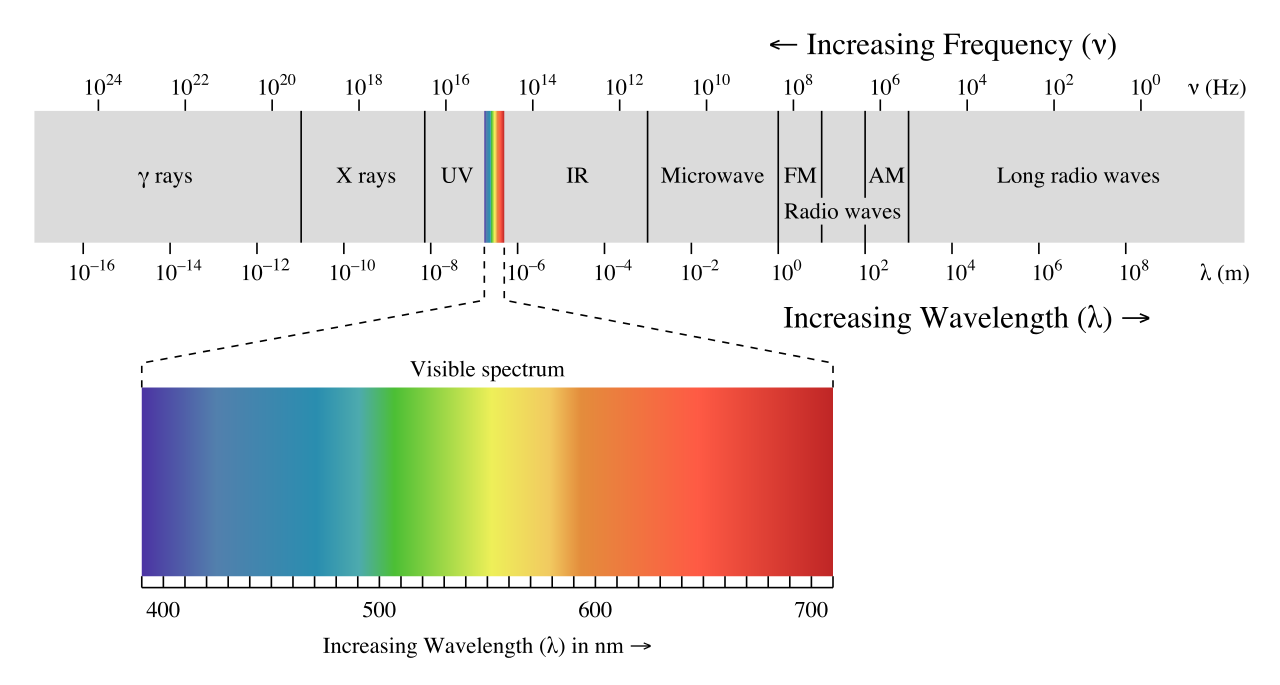
\includegraphics[width=0.7\textwidth]{images/Electromagnetic-Spectrum.png}
    \caption{The electromagnetic spectrum}
  \label{images/Electromagnetic-Spectrum.png}
\end{figure}

Electromagnetic radiation is a group of waves created by fluctuations of electric and magnetic fields radiating/propagating through space at the speed of light ($c=3\times 10^{8} m/s$) carrying electromagnetic radiant energy \citep{staats2016genetic}.\;There are numerous emission mechanisms in the universe that generate radio waves.
Each portion of the electromagnetic spectrum reveals a unique view of the universe and so modern astronomy employs various instruments to look at each portion of the spectrum.\;The Earth's atmosphere absorbs electromagnetic radiation at most infra-red, ultraviolet, X-ray, and gamma-ray wavelengths, so this allow us to only observe the universe from the ground in two windows namely the radio and visible wavebands.  Radio waves reveals objects that do not radiate in other parts of the electromagnetic spectrum and they are able to pass through galactic dust clouds that obscure the view in the optical range and able to penetrate through the earth's atmosphere (Subject to some limits depending on frequency) \citep{thompson2001interferometry}. After received by a radio telescope, the data is amplified and transferred to a computer (include figure) for further  data processing which is discussed in next chapter.


Radio astronomy was accidentally discovered by a radio Engineer, Karl Jansky in the 1930s.
Jansky was assigned the task of investigating the source of radio interference that might interfere with radio-telephone communication system at short wavelengths (10-20 meters) \citep{verschuur2015invisible}.
The purpose of this task was to find out the direction of the radio wave interference so they could easily tune out the interference by using directional antennas pointed away from the direction of the interference. In the process of conducting this task, Jansky constructed an antenna designed to receive radio waves at a frequency of 20.5 MHz (wavelength about 14.5 meters) \citep{Jansky0}. The antenna was mounted of a circular train track so that it could be rotated in all possible angles along the ground and be able to detect radio signal in all possible directions. After several months of recording and analysing these radio signals from all directions, Jansky's investigation  successfully identified two known signals (from local and  distant thunderstorms) which were interfering with the radio-telecommunication system, and one unknown signal (faint steady hiss of unknown origin). Jansky continued to investigate the third signal for over a year and he eventually figured out that the radiation was coming from the Milky Way and was strongest in the direction of the center of our Milky Way
galaxy, in the constellation of Sagittarius. This was the first detection of non-black body radiation at radio wavelengths from an extraterrestrial source. Black body radiation is the radiation given off by any object
related to its temperature \citep{Jansky1}.

After Jansky's project at Bell laboratory ended, Bell was not interested in studying astronomy any more. In 1937, an astronomer Grote Reber who was fascinated by Jansky's ground breaking discovery decided to continue where Jansky left off by further investigating the cosmic radio waves from the Milky way Galaxy. To pursue this research, Grote built the first single dish radio telescope with a receiver strong enough to detect radio cosmic signals at the back of his yard, and spent hours at night scanning the sky at different frequencies. He finally got successfully in detecting radio emission from the Milky Way Galaxy confirming Jansky's discovery \citep{verschuur2015invisible}.   

Astronomical signals tend to be weak by the time it reaches the ground, the need for greater sensitivity and higher resolution has resulted in the focus of new radio telescope development to be in the creation of telescopes that have larger collecting area for more radio energy to be focused on the receiver, external noise minimization and good quality of the receiving system to amplify the signal to levels easier to deal with \citep{verschuur2015invisible}. However constructing a single dish telescope larger enough to achieve high angular resolution $\theta \approx\frac{\lambda}{D}$ (where $\lambda$ is the wavelength of electromagnetic radiation  being observed and $D$ is the aperture diameter of the radio telescope) is physically impossible due to the cost of the materials. The angular resolution of a radio telescope measures its ability to detect fine details in the structure of the observed celestial source. For example, to obtain angular resolution of 1 arc-second, this would require a single dish radio telescope diameter to be appropriately thousands of metres \citep{verschuur2015invisible}. 

\section{Single dish vs Interferometry}
\label{RvI}
Alternatively, a single dish survey can be complemented by an array of small radio telescopes providing higher sensitivity signal and higher resolution images of features initially detected by a single dish survey \citep{wright2004single}. This technique is called radio interferometry, which is basically ensembles of two element interferometers where the incoming radio signal /wavefront from a celestial source arrive at two or more radio telescopes slightly at different times \citep{verschuur2015invisible}. The received signal from each radio telescope is combined with that from other radio telescope in the array as shown in figure \ref{images/Rint.png}. Though the telescopes are separated by distance $b$, the baseline, the resulting output is treated as one telescope. For an interferometric array the angular resolution is $\theta \approx\frac{\lambda}{B}$ where $B$ is the maximum baseline. Single dishes and interferometers  perform similar operation, they provide measurements of the Fourier transform of some region of the sky.

\begin{figure}[h!]
  \centering
    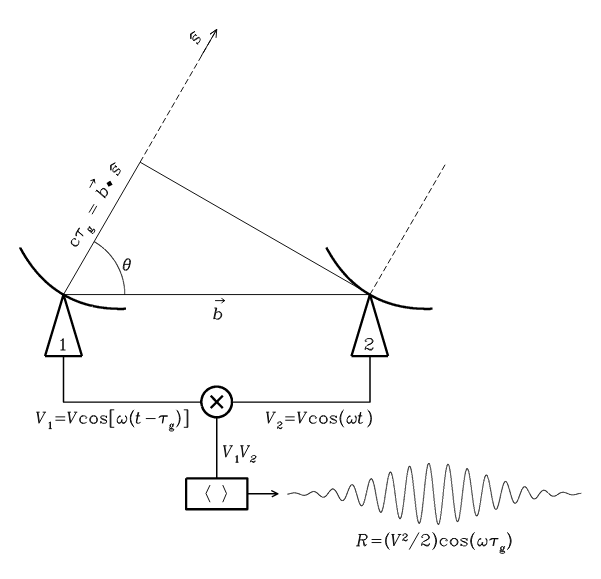
\includegraphics[width=0.45\textwidth]{images/Rint.png}
    \caption{Two antenna interferometer diagram [National Radio Astronomy Observatory]}
  \label{images/Rint.png}
\end{figure}

The figure \ref{images/Rint.png} illustrates a simple two two-element interferometer (we will refer to the left antenna as antenna 1 and the right antenna as antenna 2). This can be extended to multi-antenna arrays by replicating the antenna based portions. For an array of N-elements, there are $\frac{N(N-1)}{2}$ pair of baselines \citep{zensus1995very}. From Figure \ref{images/Rint.png}, suppose a distant star is observed in the sky, If we have two radio telescopes pointing in a direction $\widehat{s}$ at an infinitely far away source, separated by a distance $\overrightarrow{b}$, a  baseline vector from antenna 1 to antenna 2. As the wave front arrives, it will reach antenna 2 at time $\tau_{g}=\frac{\overrightarrow{b}\cdot\widehat{s}}{c}$ before it reaches antenna 1. $\tau_{g}$ is called the geometric time delay to compensate for the antenna which is further away \citep{taylor1999synthesis}. The output voltages $V_1$ and $V_2$ from both antennas is  denoted by: 

\begin{equation}\label{eq111}
\begin{split}
V_1(t)&=V\cos[\omega(t-\tau_{g})] \\
V_2(t)&=V\cos(\omega\tau_{g})
\end{split}
\end{equation}

$V_1$ and $V_2$ are then  multiplied and time averaged by the correlator to yield an output response whose amplitude R is proportional to the point-source flux density and whose phase depends on the time delay and the frequency.

\begin{align}
V_1 \times V_2 = V^2 \cos(\omega\tau_{g})\times \cos[\omega(t-\tau_{g})]
\end{align}
From $\cos A\cos B= \frac{1}{2} \left(\cos (A+B) + \cos (A-B) \right)$, 
we therefore have 
\begin{align*}
V_1 \times V_2&= \frac{V^2}{2} \left( \cos(\omega\tau_{g} + \omega t-\omega \tau_{g} )\right)\\
&= \frac{V^2}{2} \left(\cos(2\omega t - \omega \tau_{g}) + \cos (\omega\tau_{g})\right)
\end{align*}

We then take the time average $<>$ to remove the high frequency term $\cos(2\omega t - \omega \tau_{g})$ such that we obtain the output 
\begin{align}
R&= <V_1V_2> = \frac{V^2}{2}  \cos (\omega\tau_{g})\\
  &= \frac{V^2}{2}  \cos \left( \frac{\omega}{c} \overrightarrow{b} \cdot \widehat{s} \right)\\
   &= \frac{V^2}{2}  \cos \left( \frac{2\pi \nu}{c} \times
   \overrightarrow{b} \cdot \widehat{s} \right). 
\end{align}

The amplitudes $V1$ and $V2$ are proportional to the electric field produced by the  source multiplied by the the voltage gains of antennas 1 and 2.  Thus the output amplitude $\frac{V^2}{2}$ is proportional to the point-source flux density $S$ multiplied by $\sqrt{(A_1, A_2)}$, where $A_1$ and $A_2$ are the effective collecting areas of the two antennas \citep{NRAO}.

From \ref{eq111} 
Radio interferometry has enable astronomers to make measurements of  of fine angular  details including parameters such as intensity, polarization and frequency spectrum \citep{thompson2001interferometry}.

\section{Calibration in radio astronomy}
\label{Calibr}
\subsection{Interferometry Visibility}
In an interferometric array, the measured visibilities  which is the 2-dimensional Fourier transform of the sky's intensity at different baseline coordinates is defined by
\begin{align}
V(u,v)\approx \mathcal{F}\left\{I\right\}(u,v)=\int \int A(l,m) I (l,m)e^{-2\pi i(ul+vm)} dl dm,
\label{Vis}
\end{align}
where $(u,v)$ denotes the projected baseline coordinates in the 2D plane Fourier transform measured in wavelength along axes in the east-west and north south direction,  and changes with time as the earth rotates  \citep{taylor1999synthesis}. $(l, m)$ are the orthogonal coordinates representing the position of a source or the phase reference position. In the 2D analysis $l$ and $m$ are defined as the cosines of the  angles between the direction $(l,m)$ and $(u, v)$. $I(l,m)$ is the intensity distribution of a source and its Fourier transform  ${F}\left\{I\right\}$ represents the amplitude and phase of sinusoidal component of the intensity profile with spatial frequency $u$ and $v$; $A(l, m)$ represents the effective collecting area of the antennas with respect to the direction of the incoming radiation \citep{thompson2001interferometry}.

For simplicity of equation \ref{Vis}, the term $A(l,m)$ is most often assumed to be 1 such that the Van CittertZernike theorem states \citep{thompson2017interferometry}
\begin{align}
V(u,v)\approx \mathcal{F}\left\{I\right\}(u,v)=\int \int I (l,m)e^{-2\pi i(ul+vm)} dl dm.
\label{V}
\end{align}
The measured visibilities $V(u,v)$ and the sky brightness I $(l,m)$ are Fourier pairs $V(u,v) \rightleftharpoons I(l,m)$, where $\rightleftharpoons$ is the Fourier transformation. The sky
brightness can readily be recovered from the measured visibilities by an inverse Fourier transform such that we have 
\begin{align}
I(l,m)\approx \mathcal{F}^{-1}\left\{V\right\}(l,m)=\int \int V (u,v)e^{-2\pi i(ul+vm)} du dv .
\end{align}
Since for every sky's brightness $I$ $\exists$ visibility function $V(u,v)$, the array of an antennas with baseline $b=(u_i,v_i)$  measures only a certain values in the $\textbf{Set}$ of continuous  $(u,v)$ in the visibility function $V(u,v)$. This measured set of values is called \emph{Sampling function} denoted by \citep{taylor1999synthesis} \[ S(u,v) =
  \begin{cases}
    1   & \quad    \text{at uv point}\\
    0  & \quad  \text{ otherwise}\\
  \end{cases}
\], $\forall$ baselines. The actual data provided by the array is called  sampled visibilities denoted by  $S(u,v)\times V(u,v)$. The Fourier transform of this sampled visibilities is the dirty Image
\begin{align}
I^{D}(l,m)=\int \int S(u,v)\times V(u,v) e^{-2\pi i(ul+vm)} du dv.
\label{Samp}
\end{align} 
Using the $\textit{convolution theorem}$ for Fourier transforms which states that the Fourier transform of the convolution of two functions is the product of their Fourier transforms denoted by 
\begin{align}
f*g\rightleftharpoons \mathcal{F} \mathcal{G},
\end{align}
where $f\rightleftharpoons \mathcal{F}$ and $g\rightleftharpoons \mathcal{G}$.
From \ref{Samp}, we therefore have 
\begin{align}
I^{D}=PSF \circ I^{True},
\end{align}
where 
\begin{align}
PSF(l,m) = \int \int S(u,v)e^{-2\pi i(ul+vm)} du dv,
\end{align}
represents a point spread function  corresponding to the sampling function $S(u,v)$ \citep{taylor1999synthesis}.


\subsection{Calibration}
\label{Calib}
In radio astronomy, ideally one might think that after obtaining the observed visibilities the next step would be to directly retrieve the actual visibilities of the target source and perform imaging. However, in reality case it is not as simple as shown by equation \ref{V}. The measured visibilities $V^{obs}$ are different from the actual visibilities $V^{True}$ not only due to the instrument being discrete as shown in equation \ref{Samp}, but most importantly due to instrumental and environmental effects \citep{abebe2015study}. An example of these effects on the signal measured by a radio interferometry include antenna gains(slowly and fast time-varying instrumental part), atmospheric effects, pointing errors (tracking inaccuracies), Incorrect observation parameters (antenna pointing parameters). Signal effects are classified in two types; direction independent effects (affects signal from all direction of the sky) and direction dependent effects(which vary based on the sky position of the where a signal originated) \citep{taylor1999synthesis}. These effects can be corrected by estimating the errors associated with the measured visibilities, thereby recovering the true visibilities. This process is called calibration. In its simplest form, calibration boils down to minimizing the difference between observed and predicted(model) visibilities by estimating the complex instrumental gain response \citep{grobler2016calibration}. 

Suppose for baseline pair $(i,j)$, the observed visibility is $V^{obs}_{i,j}(t)$ and the true visibility is $V^{True}_{i,j}(t)$ at observation time $t$. The basic calibration formula is written as 

\begin{align}
V_{i,j}^{obs}=G_{i,j} V_{i,j}^{true} + \epsilon_{i,j}(t) ,
\end{align}
where $G_{i,j}(t)$ denote the complex antenna gains for baseline $(i,j)$ as a results of unwanted effects and may vary with time \citep{thompson2001interferometry}. The extra term $ \epsilon_{i,j}(t)$ is a stochastic complex noise \citep{taylor1999synthesis}.

Since most of the corruptions in data occurs before the signal gets correlated and the response associated with antenna  $i$  does not depend on the response of antenna $j$. Then the baseline-based complex gain $G_{i,j}$ can therefore be approximated into the product of amplitude and phase $A$ and phase $\phi$ such that we have  

\begin{align}
G_{i,j}(t)= g_i(t)g^*_j(t) = A_{i}(t)A_{j}(t) e ^{i\left(\phi_i(t)-\phi_j(t)\right)},
\label{Sols}
\end{align}

where  $A_{i}(t)$, $A_{j}(t)$ are antenna-based amplitude solutions and $\phi_i(t),\phi_j(t)$ are antenna-based phase solutions. Calibration means to find the appropriate $A$ and $\phi$ for the corrupted visibilities. One standard technique of obtaining solutions to \ref{Sols} is to obtain dedicated calibration observations of a part of the sky that contains a single known, relatively strong point source. The reason for observing these sources is to measure the instrumental phase since the telescopes on the ground can only measure the phase differences rather than measuring absolute phase reference. Therefore, the reference for phase visibility to the phase tracking center or the center of the primary antenna beam can be practically accomplished by observing point-like calibrator sources, the phase . Using these sources, one can determine the phase deviation from the desired reference point. Periodic observation of these sources is very important so as to track the phase and gain changes in an array. Above all, they have the paramount advantage to estimate time dependent phase changes incurred by the atmosphere \citep{taylor1999synthesis}.

The selection of a good calibrator source in the sky is based on the following desirable characteristics \citep{thompson2001interferometry} 

\begin{enumerate}
\item They should have known positions in the sky, i.e the calibrator should be close to the target source. 
\item  Their flux densities have to be strong enough so as to get suitable signal-to-noise ratio (SNR) for calibrating in a short time.
 \item The calibrator should be a point source (unresolved) if possible. 
 \item Their spectral properties should be known.
 \end{enumerate}
 
 Note that the source that is the subject  of the astronomical investigation will be referred to as target sources to distinguish them from the calibrator sources \citep{thompson2001interferometry}.
 
Supposed a target source is observed with measured visibility $V(u,v)^{obs}$. To calibrate the antenna-based complex gain factor $G_{i,j}(t)$ as a function of time and antenna pair (i,j), a point source calibrator is observed for which the measured visibility is 
\begin{align}
V(u,v)_{calibrator}&= G_{i,j}(t) S_{calibrator}\\
G_{i,j}(t)&= \frac{V(u,v)_{calibrator}}{S_{calibrator}},
\citep{thompson2001interferometry}
\end{align}
where S indicates the flux density of the calibrator. Now to calibrate the visibilities of the target source we can write  
\begin{align}
V(u,v)^{true}&= \frac{V(u,v)^{obs}}{G_{i,j}(t)}\\
&= V(u,v)^{obs} \times \frac{S_{calibrator}}{V(u,v)_{calibrator}}
\citep{thompson2001interferometry}  
\end{align}

\section{Calibration techniques}
\label{caltech}
With the improvement and complexities of the new radio astronomy instruments, various calibration techniques have been developed to overcome these challenges  posed by the new instruments thereby producing accurate calibration results. These techniques are classified into first generation calibration (1GC), second generation calibration (2GC) and third generation calibration (3GC). In this thesis our focus will be on 1GC using the Common Astronomy Software Applications (CASA) which is a suit of functions for the reduction and analysis of radio astronomical data with IPython interface, and is currently maintained by the National Radio Astronomy Observatory \citep{mcmullin2007casa}. 

\subsection{First generation calibration(1GC)}

This is the first step in data reduction process where in simple, the received signal in each baseline is compared to the signal from a known source (the calibrator sources) to address the following errors in the response of the instrument. 

\begin{itemize}

\item Bandpass calibration B is used to solve for gain variations
in frequency. Variation in frequency arises as a result of non-uniform filter passbands or other frequency dependent effects in signal transmission. It is usually the case that these frequency-dependent effects vary on timescales much longer than the time-dependent effects. The casa task which solves these frequency dependant complex gains is called $\textit{bandpass}$. This is done by observing a strong calibrator source with a known model visibilities and spectrum characteristics for sufficient time to reach the required accuracy \citep{taylor1999synthesis}.

\item Delay calibration K is used to correct for the phase delay errors. Since the arriving signal does not propagate all the antennas at the same time. Delay calibration equalizes these propagation difference on individual signal path at the input of the correlator and removes the largest phase difference across the observing band \citep{taylor1999synthesis}.   

\item Gain calibration G is used to solve for time dependant complex gain variation. These gain variations includes the relative amplitude and phase gain for each antenna, phase and amplitude drifts in the electronics of each antenna, amplitude response as a function of elevation (gain curve), and tropospheric amplitude and phase effects. Some of these calibrations are known beforehand (“a priori”)and others must be determined from observations of calibrator sources. The casa task used to solves for these antenna-based gains in each polarization in specified time solution intervals  is $\textit{gaincal}$ \citep{editioncasa}.  

Note that it is not always possible to find a calibrator source that satisfies the requirements mentioned in \ref{Calib}, especially point number 2. In such cases it may be necessary to find a calibrator source that is a point source  close to the target source and the calibrate it against one of the more commonly used flux density reference calibrators such as PKS1934-638, 3C147, 3C286 \citep{thompson2001interferometry}. 

\item Flux calibration is used to calibrate the flux density of source calibrators with unknown flux densities. The flux density of the unknown calibrators is assumed to be 1Jy such that the complex gain solutions G of the reference flux density calibrator and one with unknown flux density are compared and scaled so that they match as much as possible. The casa task used to perform this scaling or bootstrapping is $\textit{fluxscale}$ \citep{editioncasa}.
\end{itemize}

The solutions obtained from the tasks ($\textit{gaincal}$, $\textit{bandpass}$, $\textit{fluxscale}$) are saved in tables and then later be applied on uncalibrated data 
to form calibrated data.

\subsection{Second generation calibration(2GC)}

Once the calibrated data is obtained by performing the first generation calibration and the first model image is computed. A process called self calibration can be performed to obtain more accurate images by making additional corrections to the antenna gains as a function of time. It is very similar to the basic calibration. The main difference is that the model of the source is generally more complex than just assuming its a point source at the phase centre and also the observed field is used to calibrate itself \citep{wieringa1992investigation}. The self-calibration technique finds antenna gains $g_i$, which minimise the difference between the measured visibilities $V_{i,j}$, and the model visibilities $\hat{V}_{i,j}$ \citep{grobler2016calibration}, 

\begin{align}
\epsilon^2 = \sum |V_{i,j}-g_i g_j^* V^{obs}_{i,j}|^2
\label{ls}
\end{align}

Self calibration can be briefly described using the flowchart in Figure \ref{self},
\begin{figure}[H]
  \centering
    \includegraphics[width=0.7\textwidth]{images/Selfcal.png}
    \caption{Selfcal flow diagram} 
    \label{self} 
\end{figure}

and can be performed using the following method:
\begin{enumerate}
\item Create an initial source model from an initial image (1GC).
\item Set your model to the initial skymodel and use it to find antenna gains using least squares as shown in equation \ref{ls}.
\item Apply gains to the observed visibilities.
\item 3. Image the corrected visibilities and create new model visibilities. 
\item Return to Step 2 with your new skymodel or terminate if the current model is satisfactory.
\end{enumerate}
\subsection{Third generation calibration(3GC)}

The First and Second generation calibration discussed in the previous sections focused mainly on solving direction independent effects. With the wide field of views of current and future generation of radio telescopes such as Extended Very Large Array, Low Frequency Array and the SKA, direction dependent effects poses a challenge in calibration which result into the third generation calibration (3GC). 3GC is the family of new calibration techniques for dealing with direction-dependent effects. These are effects that vary not only with time and frequency but also the viewing direction \citep{pandey2009calibrating}. This include variations in the primary beam or sensitivity pattern of each antenna. 